\documentclass[10pt]{article}

\usepackage{amsmath}
\usepackage{fullpage}
\usepackage{array}
\usepackage{graphicx}
\usepackage{gensymb}
\usepackage{booktabs}
\usepackage{gensymb}
\usepackage{graphicx}
\usepackage{hyperref}
\hypersetup{colorlinks,urlcolor=blue}
\usepackage{mathtools}


\graphicspath{ {../Images/} }

\date{2014-6-22}
\pagestyle{empty}
\setlength{\parindent}{0pt}

\begin{document}
\begin{center}
\begin{Large}\textbf{Chapter: Fluids}\end{Large} \\
\smallskip
%\begin{large} Acceleration \end{large}
\end{center}
%%%%%%%
Objectives: Define fluids with their properties, applications of Archimedes' principle.
\section{Fluids}
A \emph{fluid} is a substance that has no fixed shape and, thus, it can flow.  Fluids conform to the boundaries of any container in which they are put.  The reason is that they cannot sustain a force that is tangential to their surface.  However, fluids can exert a force in the direction perpendicular to their surface.  Liquids and gases are the two examples of fluid.
\subsection{Pressure}
Pressure is defined as the perpendicular force per unit area.  
\begin{equation}
  p=\frac{F}{A}
\end{equation}
where $F$ is the magnitude of the normal force on the area $A$.  The SI unit of pressure is the newton per square meter or pascal (Pa).
\subsection{Density}
Density is defined as mass per unit volume
\begin{equation}
  \rho = \frac{m}{V}
\end{equation}
and the units are kg.m/$\text{sec}^2$.  

\section{Archimedes' Principle}
The principle states that when a body is fully or partially submerged in a fluid, the fluid pushes upward with a bouyant force with the magnitude
\begin{equation}
\label{bouyequation}
  F_b=m_fg
\end{equation}
where $m_f$ is the mass of the \emph{fluid} displaced by the submerged body and $g$ is the acceleration due to gravity.

Thus in order for a body to float, the bouyant force must be equal to the weight of the body.  Consider a student in a swimming pool with a thin bag filled with the same water as shown 
\begin{figure}[h]
\label{studentswimmer}
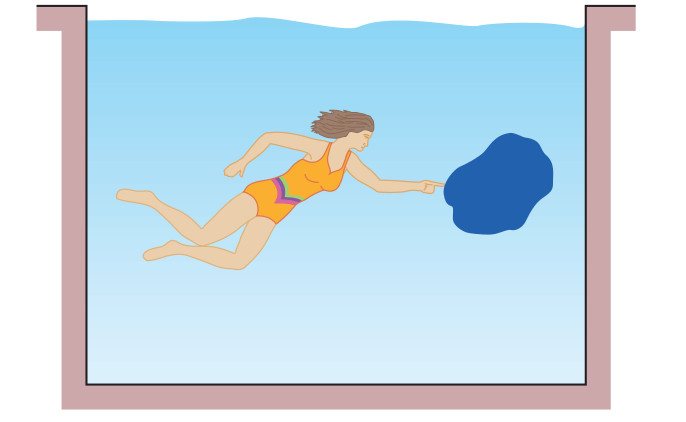
\includegraphics[scale=.7]{studentswimmer}
\centering
\caption{Student with a bag filled with water}
\centering
\end{figure}
She observes that the sack and its contained water are in static equilibrium, tending neither to rise nor to sink.  It means that the downaward gravitational force $\vec{F}_g$ on the contained water must be balanced by a net upward force from the water surrounding the sack.  We call this force the \emph{bouyant} force, $\vec{F}_b$.  It exists because the pressure near the bottom of the sack is greater than that in the top.  The figure \ref{bouymagforce} gives a good estimate of the force magnitude resulting from the pressure in water.
\begin{figure}[h]
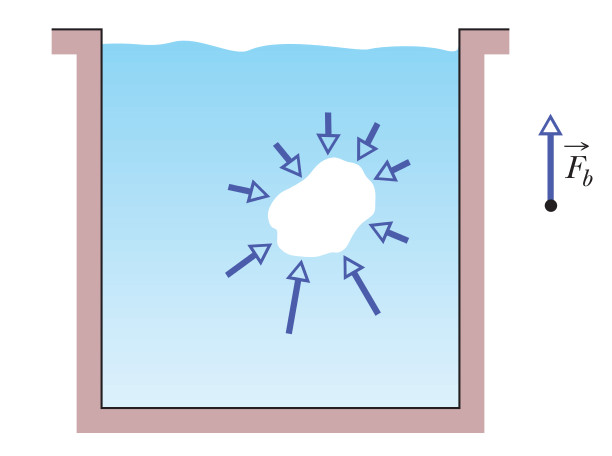
\includegraphics[scale=.7]{forcemagbouy}
\centering
\caption{The bouyant force due to surrounding water}
\label{bouymagforce}
\centering
\end{figure}
The magnitude of the bouyant force is given by equation \ref{bouyequation}.

On the other hand, if the object sinks in the water, then the \emph{effective} weight of the object is reduced by the amount which is equal to its \emph{bouyant} force.  Thus
\begin{equation}
  \text{weight}_{\text{app}}=\text{weight} - F_b
\end{equation}

\section{Sample problems}
\begin{enumerate}
\item In the figure \ref{blockfloat}, a block of density $\rho = 800$ kg/$\text{m}^3$ floats face down in a fluid of density $\rho_f = 1200$ kg/$\text{m}^3$.  The block has height $H=6$ cm.
  \begin{enumerate}
  \item By what depth $h$ is the block submerged?
  \item If the block is held fully submerged and then released, what is the magnitude of its acceleration?
  \end{enumerate}
\begin{figure}[h]
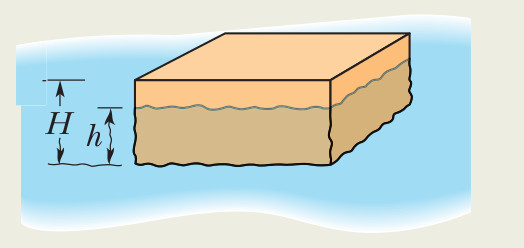
\includegraphics[scale=.9]{partialfloat}
\centering
\caption{A body partially submerged in water}
\label{blockfloat}
\centering
\end{figure}
\vspace{300px}
\item In figure \ref{suspenblock} the cube of edge length $L=0.600$ m and mass 450 kg is suspended by a rope in an open tank of liquid of density 1030 kg/$\text{m}^3$.  Find 
  \begin{enumerate}
  \item the tension in the rope
  \item magnitude of the bouyant force on the cube using Archimedes' principle.
  \end{enumerate}
\begin{figure}[h]
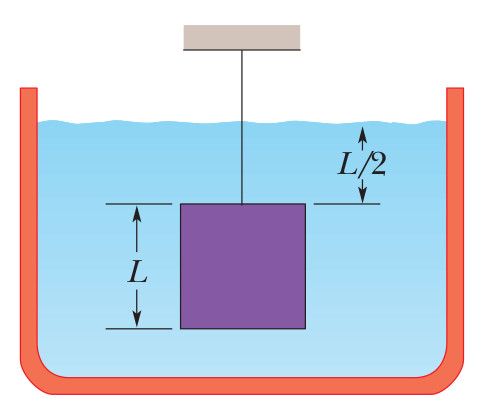
\includegraphics[scale=.9]{suspendedblock}
\centering
\caption{A block suspended in water}
\label{suspenblock}
\centering
\end{figure}
\end{enumerate}
\end{document}
